\def\mytitle{LINES ASSIGNMENT}
\def\myauthor{PANJUGALA SHASHIKALA}
\def\contact{sashipanjugala@gmail.com}
\def\mymodule{Future Wireless Communication (FWC)}
\documentclass[10pt, a4paper]{article}
\usepackage[a4paper,outer=1.5cm,inner=1.5cm,top=1.75cm,bottom=1.5cm]{geometry}
\twocolumn
\usepackage{setspace}
\doublespacing
\usepackage{graphicx}
\graphicspath{{./images/}}
\usepackage[colorlinks,linkcolor={black},citecolor={blue!80!black},urlcolor={blue!80!black}]{hyperref}
\usepackage[parfill]{parskip}
\usepackage{lmodern}
\usepackage{tikz}
	\usepackage{physics}
%\documentclass[tikz, border=2mm]{standalone}
\usepackage{karnaugh-map}
%\documentclass{article}
\usepackage{tabularx}
\usepackage{circuitikz}
\usetikzlibrary{calc}
\usepackage{amsmath}
\usepackage{amssymb}
\renewcommand*\familydefault{\sfdefault}
\usepackage{watermark}
\usepackage{lipsum}
\usepackage{xcolor}
\usepackage{listings}
\usepackage{float}
\usepackage{titlesec}
\providecommand{\mtx}[1]{\mathbf{#1}}
\titlespacing{\subsection}{1pt}{\parskip}{3pt}
\titlespacing{\subsubsection}{0pt}{\parskip}{-\parskip}
\titlespacing{\paragraph}{0pt}{\parskip}{\parskip}
\newcommand{\figuremacro}[5]{
    \begin{figure}[#1]
        \centering
        \includegraphics[width=#5\columnwidth]{#2}
        \caption[#3]{\textbf{#3}#4}
        \label{fig:#2}
    \end{figure}
}
\newcommand{\myvec}[1]{\ensuremath{\begin{pmatrix}#1\end{pmatrix}}}
\let\vec\mathbf
\lstset{
frame=single, 
breaklines=true,
columns=fullflexible
}

\thiswatermark{\centering \put(-15,-100.0){
\includegraphics[scale=0.4]{iith.png}} }
\title{\mytitle}
\author{\myauthor\hspace{1em}\\\contact\\FWC22097 -\hspace{0.5em}IITH\hspace{0.5em}\mymodule\hspace{6em}}
\date{}
\begin{document}
	\maketitle
	\tableofcontents
   \section{Problem}
 If a vertex of a triangle is (1,1) and the midpoints of two sides through this vertex are (-1,2) and (3,2). Then find the centroid of the triangle.

	   % 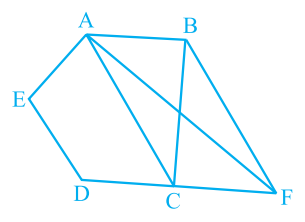
\includegraphics[scale=1.0]{diag_1.png}
   \section{Solution}

Let A,B and C be the vertices of the triangle. And E , F are midpoints of two sides through the vertex A.
Given $\vec{A}=(1,1), \vec{E}=(-1,2), \vec{F}=(3,2)$ 
\begin{center}
%\begin{tabular}{|c|c|}
%	\textbf{Symbol}&\textbf{Value}\\
%	\hline
%	b&6\\
%	\hline
%	r&5\\
%	\hline
%	$\theta$&$\frac{\pi}{3}$\\
%	\hline
%\end{tabular}
%\begin{center}
$\vec{A}=\myvec{ 1 \\ 1 }$\\
$\vec{E}=\myvec{-1 \\ 2 }$\\
$\vec{F}=\myvec{ 3 \\ 2 }$\\
Midpoint of a triangle is 
$$ \vec{M}=\frac{\vec{A}+\vec{B}}{2}$$

By using the above formula, we can find the other two vertices as
$$\vec{B}=2\left(\vec{E}-\frac{1}{2}\vec{A}\right)$$

$\vec{B}=\myvec{-3 \\ 3 }$\\

$$\vec{C}=2\left(\vec{F}-\frac{1}{2}\vec{A}\right)$$

$\vec{C}=\myvec{ 5 \\ 3 }$\\
\end{center}
%\end{center}

We can find the centroid by using three vertices A,B and C.
\textbf{Centroid:} 
		\begin{center}
		
		Centroid $\vec{G}=\frac{(\vec{A}+\vec{B}+\vec{C})}{3}$
		
		By substituting the vertices in above formula we get centroid as
		 
		$\vec{G}=\myvec{ 1 \\ 7/3}$\\
	\end{center}
 
 
 \section{Construction}
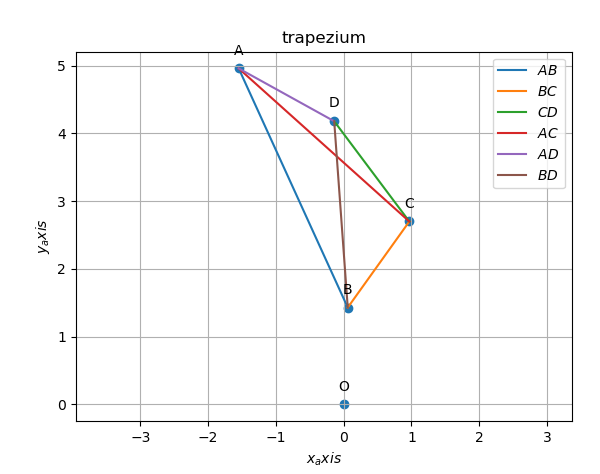
\includegraphics[scale=0.5]{line.png}



\section{Software}


The below python code realizes the above construction:	\\
\begin{lstlisting}
https://github.com/PanjugalaShashikala/FWC_2022097/tree/main/Lines
 \end{lstlisting}
 	

%\bibliographystyle{ieeetr}
\end{document}
